%% The following is a directive for TeXShop to indicate the main file
%%!TEX root = diss.tex

\chapter{Lexical decision}
\label{chap:lexdec}

\section{Motivation}

The experiments in this chapter implement a standard lexically-guided perceptual learning experiment with exposure to a modified /s/ category during a lexical decision task.
Because the exposure task is one of word recognition, participants are predicted to default to a comprehension-oriented attentional set.  
Recall that comprehension-oriented attentional sets are hypothesized to facilitate perceptual learning and generalization.
Two experimental manipulations guide listeners to use more of  a perception-oriented attentional set.
The first manipulation relates to the position of the modified /s/ category in the exposure tokens (\emph{silver} versus \emph{carousel}).
Exposure to an ambiguous category in a position of less lexical bias 
Lexical bias effects increase as the length of the word increases and as the word unfolds \citep{Pitt2006, Pitt2012}, so we predict that more learning will take place in \emph{carousel}-like words.
The second manipulation is through explicit instructions about the modified /s/ category.
Such instructions have been shown to reduce lexical bias effects in lexical decision tasks \citep{Pitt2012}, thus we predict a reduction in learning when attention is drawn to speech sounds.
Both of these manipulations will be present in Experiments 1 and 2.

Experiments 1 and 2 differ in how typical the modified /s/ category.
Studies have reported greater perceptual learning when ambiguous stimuli are closer to the distribution expected by a listener than when the ambiguous stimuli are farther away from expected distributions \citep{Sumner2011}.  
Words containing stimuli farther away from the target production are in general less likely to be endorsed as words, but similar effects of attention are found across word position \citep{Pitt2012}.  
Experiment 2 contains the same manipulations to attention and lexical bias as Experiment 1, but with ambiguous stimuli farther from the target production than those used in Experiment 1.
Lower rates of generalized perceptual learning are predicted for all conditions in Experiment 2.

The hypothesis of this dissertation predicts that the greatest perceptual learning effects should be observed when no attention is directed to the ambiguous sounds and when lexical bias is maximized.  
In such a case, participants should use a comprehension-oriented attentional set.  
If selective attention is directed to the ambiguous sounds, a more perception-oriented attentional set should be adopted with less generalization in perceptual learning as a result. 
Likewise, if the ambiguous sound is in a linguistically salient position with little to no lexical bias, a listener's attention should be drawn to the ambiguous sound, causing adoption of a more perception-oriented attentional set.  
Finally, if the ambiguous sounds are more atypical, they should be more salient to listeners regardless of lexical bias, leading again to a more perceptual oriented attentional set.  
Regardless of the cause, adopting a perception-oriented attentional set is predicted to inhibit a generalized perceptual learning effect.

\section{Experiment 1}

In this experiment, listeners are exposed to ambiguous productions of words containing a single instance of /s/, where the /s/ has been modified to sound more /\textesh/-like.
Exposure comes in the guise of a lexical decision task. 
In one group, the critical words have an /s/ in word-initial position (\emph{cement}), with no /\textesh/ neighbor (\emph{shement}); this is referred to as the Word-initial condition.  
In the other group, the critical words will have an /s/ in word-medial position (\emph{tassel}) with no /\textesh/ neighbor (\emph{tashel}); this is referred to as the Word-medial condition.  
In addition, half of each group will be given instructions that the speaker has an ambiguous /s/ and to listen carefully, following \citet{Pitt2012}.

Given the difference in word response rates based on position in the word \citep{Pitt2012}, we predict that listeners exposed to ambiguous sounds earlier in words will be less likely to accept these productions as words as compared to listeners exposed to ambiguous sounds later in words.  
In addition, given the reliance of perceptual learning on lexical scaffolding, this lower acceptance rate for the Word-initial group should lead to a smaller perceptual learning effect as compared to the Word-medial group.

\subsection{Methodology}

\subsubsection{Participants}

A total of 173 participants from the UBC population completed the experiment and were compensated with either \$10 CAD or course credit.  
The data from 77 non-native speakers of English and two native speakers of English with reported speech or hearing disorders were excluded from the analyses.
This left data from 94 participants for analysis.
Twenty additional native English speakers participated in a pretest to determine the most ambiguous sounds.  
Twenty-five other native speakers of English participated for course credit in a control experiment.

\subsubsection{Materials}

\begin{table}[ht]
\caption{Filler words used in all experiments.}
\label{tbl:fillerwords}
\centering
\begin{tabular}{cccccc}
\toprule
acorn       & acrobat   & antenna   & apple     & balloon  & bamboo     \\
buckle      & butterfly & cabin     & calendar  & camel    & campfire   \\
candy       & cockpit   & collar    & cowboy    & cradle   & cutlery    \\
darkroom    & diamond   & doorbell  & dryer     & elephant & feather    \\
fingerprint & garlic    & goalie    & gondola   & graffiti & helicopter \\
ladder      & ladle     & librarian & lightning & lumber   & mannequin  \\
meadow      & microwave & minivan   & motel     & movie    & mural      \\
napkin      & omelet    & painter   & piano     & ponytail & popcorn    \\
referee     & table     & tadpole   & teapot    & theatre  & tire       \\
tortilla    & tractor   & traffic   & tunnel    & umbrella & weatherman\\
\bottomrule
\end{tabular}
\end{table}

\begin{table}[ht]
\caption{Filler nonwords used in Experiments 1 and 2.}
\label{tbl:fillernonwords}
\centering
\begin{tabular}{cccccc}
\toprule
apolm     & arafimp    & arnuff       & balrop   & bambany     & bawapeet  \\
bettle    & bimobel    & bipar        & blial    & brahata     & danoor    \\
darnat    & deoma      & follipocktel & foter    & gallmit     & gamtee    \\
ganla     & gippelfraw & giptern      & gittle   & glaple      & golthin   \\
goming    & gompy      & gorder       & hagrant  & hammertrent & hintarber \\
hovear    & iddle      & iglopad      & igoldion & impomo      & inoret    \\
kempel    & kimmer     & kire         & klogodar & kowack      & lefeloo   \\
lindel    & mogmet     & mopial       & motpem   & namittle    & nartomy   \\
nepow     & neproyave  & nidol        & noler    & nometin     & nonifem   \\
omplero   & pammin     & peltlon      & pickpat  & pidbar      & pluepelai \\
poara     & poltira    & pomto        & potha    & prickpor    & prithet   \\
radadub   & rigloriem  & rinbel       & rindner  & ripnem      & roggel    \\
roppet    & rudle      & talell       & talot    & tankfole    & tayade    \\
teerell   & tello      & tepple       & teygot   & theely      & theerheb  \\
thorkwift & thragkole  & timmer       & tingora  & tinogail    & tirack    \\
tirrenper & tovey      & toygaw       & tuckib   & tuddom      & tutrewy   \\
wapteep   & wekker     & wogim        & yovernon &             &          \\
\bottomrule
\end{tabular}
\end{table}

One hundred and twenty English words and 100 phonologically-legal nonwords were used as exposure materials.  
The set of words consisted of 40 critical items, 20 control items, and 60 filler words.  
Filler words and nonwords are listed in Tables~\ref{tbl:fillerwords} and~\ref{tbl:fillernonwords}, respectively.
The control words containing /\textesh/ are given in Table~\ref{tbl:shwords}.
Half of the critical items had an /s/ in the onset of the first syllable (Word-initial) and half had an /s/ in the onset of the final syllable (Word-medial).  
All critical tokens formed nonwords if their /s/ was replaced with /\textesh/. Half the control items had an /\textesh/ in the onset of the first syllable and half had an /\textesh/ in the onset of the final syllable.  
Each critical item and control item contained just the one sibilant, with no other /s z \textesh\ \textyogh\ \textteshlig\  \textdyoghlig/.  
Filler words and nonwords did not contain any sibilants.  
Frequencies and number of syllables across item types are in Table~\ref{tbl:expfreq}

\begin{table}[ht]
\caption{Words containing /\textesh/ in all experiments.}
\label{tbl:shwords}
\centering
\begin{tabular}{cccc}
\toprule
auction & brochure & cashier     & chandelier  \\
cushion & eruption & hibernation & parachute   \\
patient & shadow   & shampoo     & shareholder \\
shelter & shiny    & shoplifter  & shoulder    \\
shovel  & sugar    & tissue      & usher      \\
\bottomrule
\end{tabular}
\end{table}

\begin{table}[ht]
\caption{Mean and standard deviations for frequencies (log frequency per million words in SUBTLEXus) and number of syllables of each item type}
\label{tbl:expfreq}
\centering
\begin{tabular}{ccc}
\toprule
Item type & Frequency & Number of syllables \\
\midrule
Filler words & 1.81 (1.05) & 2.4 (0.55) \\
/s/ Word-initial & 1.69 (0.85)  & 2.4 (0.59)\\
/s/ Word-medial & 1.75 (1.11)  & 2.3 (0.47) \\
/\textesh/ Word-initial & 2.01 (1.17) & 2.3 (0.48) \\
/\textesh/ Word-medial & 1.60 (1.12) & 2.4 (0.69) \\
\bottomrule
\end{tabular}
\end{table}

Four monosyllabic minimal pairs were selected as test items for categorization.
These minimal pairs differed only in the voiceless sibilant at the beginning of the word (\emph{sack}-\emph{shack}, \emph{sigh}-\emph{shy}, \emph{sin}-\emph{shin}, and \emph{sock}-\emph{shock}).  
Two of the pairs had a higher log frequency per million words (LFPM) from SUBTLEXus \citep{Brysbaert2009} for the /s/ word and two had higher LFPM for the /\textesh/ word, as shown in Table~\ref{tbl:catfreq}.

\begin{table}[ht]
\caption{Frequencies (log frequency per million words in SUBTLEXus) of words used in categorization continua}
\label{tbl:catfreq}
\centering
\begin{tabular}{ccc}
\toprule
Continuum & /s/-word frequency & /\textesh/-word frequency \\
\midrule
sack-shack & 1.11 & 0.75 \\
sigh-shy & 0.53 & 1.26 \\
sin-shin & 1.20 & 0.48 \\
sock-shock & 0.95 & 1.46 \\

\bottomrule
\end{tabular}
\end{table}


All words and nonwords were recorded by a male Vancouver English speaker in quiet room.  
Critical words for the exposure phase were recorded in pairs, once normally and once with the sibilant swapped forming a nonword.  
The speaker was instructed to produce both forms with comparable speech rate, speech style, and prosody.

For each critical item, the word and nonword versions were morphed together in an 11-step continuum (0\%-100\% of the nonword /\textesh/ recording, in steps of 10\%) using STRAIGHT \citep{Kawahara2008} in Matlab.  
Prior to morphing, the word and nonword versions were time aligned based on acoustic landmarks, such as stop bursts, onset of F2, nasalization or frication, etc.  
All control items and filler words were processed and resynthesized by STRAIGHT to ensure a consistent quality across stimulus items.

\subsubsection{Pretest}

To determine which step of each continua would be used in exposure, a phonetic categorization experiment was conducted.  
Participants were presented with each step of each exposure word-nonword continuum and each categorization minimal pair continuum, resulting in 495 trials (40 exposure words plus five minimal pairs by 11 steps).  
The experiment was implemented in E-prime \citep{PsychologySoftwareTools2012}.  

\begin{figure*}[ht]
\caption{Proportion of word-responses for Word-initial exposure words. Solid lines represent Experiment 1 selection criteria (50\% word-response rate) and dashed lines represent Experiment 2 selection criteria (30\% word-response rate).  Dots are averaged word-response across subjects, and the blue line is a binomial model of the responses.}
\label{fig:sinitialpretest}
\begin{center}
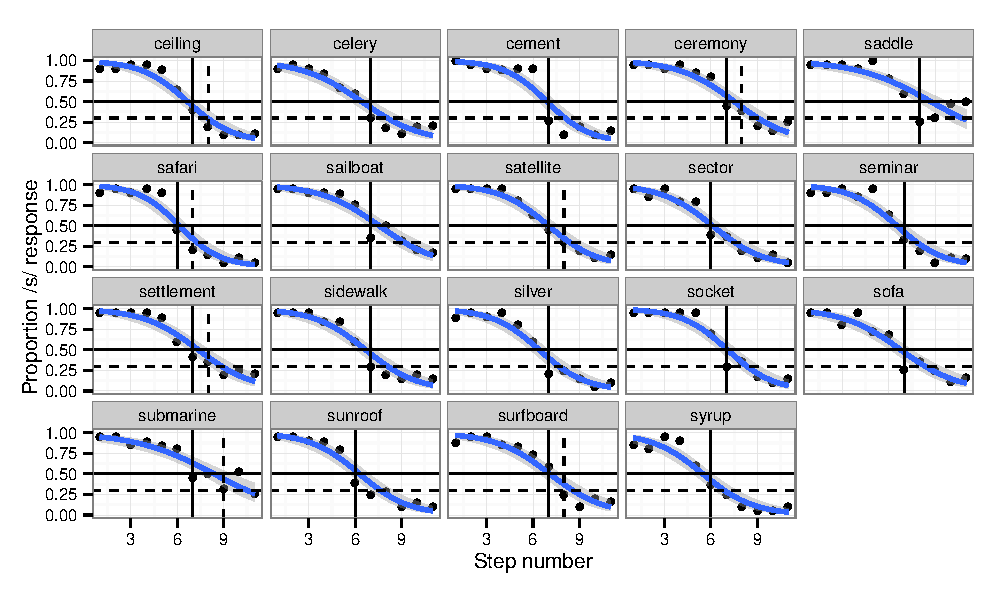
\includegraphics[width=\textwidth]{graphs/sinitialpretest.pdf}
\end{center}
\end{figure*}

\begin{table}[ht]
\caption{Step chosen for each Word-initial stimulus in Experiment 1 and the proportion /s/ response in the pretest}
\label{tbl:exp1srespinitial}
\centering
\begin{tabular}{ccc}
\toprule
Word & Step chosen & Proportion /s/ response \\
\midrule
 ceiling & 7 & 0.40 \\
celery & 7 & 0.30 \\
cement & 7 & 0.26 \\
ceremony & 7 & 0.44 \\
saddle & 8 & 0.25 \\
safari & 6 & 0.45 \\
sailboat & 7 & 0.35 \\
satellite & 7 & 0.45 \\
sector & 6 & 0.39 \\
 seminar & 7 & 0.33 \\
 settlement & 7 & 0.42 \\
 sidewalk & 7 & 0.30 \\
 silver & 7 & 0.21 \\
 socket & 7 & 0.30 \\
 sofa & 7 & 0.26 \\
 submarine & 7 & 0.45 \\
 sunroof & 6 & 0.39 \\
 surfboard & 7 & 0.59 \\
 syrup & 6 & 0.37 \\
\midrule
 Average &  6.8 & 0.36 \\

\bottomrule
\end{tabular}
\end{table}

The proportion of /s/-responses (or word responses for exposure items) at each step of each continuum was calculated and the most ambiguous step chosen. 
The threshold for the ambiguous step for Experiment 1 was when the percentage of /s/-response dropped near 50\%. 
The lists of steps chosen for Word-initial target stimuli is in Table~\ref{tbl:exp1srespinitial} and Table~\ref{tbl:exp1srespfinal}, respectively.
For the minimal pairs, six steps surrounding the 50\% cross-over point were selected for use in the phonetic categorization task.  
Due to experimenter error, the continuum for \emph{seedling} was not included in the stimuli, so the chosen step was the average chosen step for the /s/-initial words.  
The average step chosen for Word-initial /s/ words was 6.8 ($SD = 0.5$), and for Word-medial /s/ words the average step was 7.7 ($SD = 0.8$).


\begin{figure*}[ht]
\caption{Proportion of word-responses for Word-medial exposure words. Solid lines represent Experiment 1 selection criteria (50\% word-response rate) and dashed lines represent Experiment 2 selection criteria (30\% word-response rate).  Dots are averaged word-response across subjects, and the blue line is a binomial model of responses.}
\label{fig:sfinalpretest}
\begin{center}
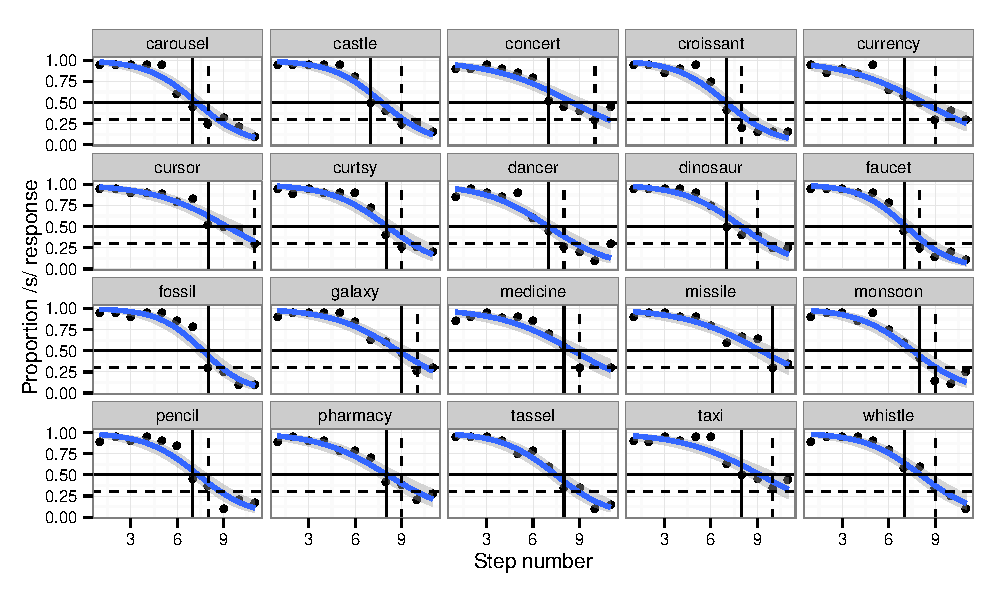
\includegraphics[width=\textwidth]{graphs/sfinalpretest.pdf}
\end{center}
\end{figure*}


\begin{table}[ht]
\caption{Step chosen for each Word-medial stimulus in Experiment 1 and the proportion /s/ response in the pretest}
\label{tbl:exp1srespfinal}
\centering
\begin{tabular}{cccc}
\toprule
 Word & Step chosen & Proportion /s/ response \\
\midrule
carousel & 7 & 0.45 \\
castle & 7 & 0.50 \\
concert & 7 & 0.53 \\
croissant & 7 & 0.42 \\
currency & 7 & 0.58 \\
cursor & 8 & 0.53 \\
 curtsy & 8 & 0.40 \\
 dancer & 7 & 0.45 \\
 dinosaur & 7 & 0.50 \\
 faucet & 7 & 0.45 \\
 fossil & 8 & 0.30 \\
 galaxy & 9 & 0.47 \\
 medicine & 8 & 0.55 \\
 missile & 10 & 0.30 \\
 monsoon & 8 & 0.42 \\
 pencil & 7 & 0.45 \\
pharmacy & 8 & 0.42 \\
tassel & 8 & 0.35 \\
 taxi & 8 & 0.50 \\
 whistle & 7 & 0.58 \\
\midrule
 Average   & 7.7 & 0.45 \\

\bottomrule
\end{tabular}
\end{table}

To visualize the effect of morphing on the acoustics of the sibilants and to confirm the desired effects, a multidimensional scaled plot of acoustic distance was constructed.  
Using the \texttt{python-acoustic-similarity} package \citep{McAuliffe2015}, sibilants were transformed into arrays of mel-frequency cepstrum coefficients (MFCC), and then pairwise distances were computed via dynamic time warping to create a distance matrix of the sibilant productions.  
This distance matrix was then multidimensionally scaled to produce Figure~\ref{fig:exp1mds}.  
As seen there, the original, unsynthesized productions (in blue) form four quadrants based on the two principal components of the distance matrix. 
 The first dimension is associated with the centroid frequency of the sibilant, separating /s/ tokens from /\textesh/.  
The second dimension separates out the word-medial sibilants (in smaller font) from the word-initial sibilants (in larger font), likely due to the different coarticulatory effects based on word position.  
The categorization tokens (all word-initial) predictably occupy the space between the word-initial /s/ tokens and the word-initial /\textesh/ tokens. 
 The exposure tokens pattern as expected.  Exposure /\textesh/ tokens are overlapping with the original distributions for /\textesh/ tokens.  
Exposure /s/ tokens are in between /s/ and /\textesh/, though word-medial /s/ tokens are closer to the original /\textesh/ distribution, reflecting the difference in average stimuli step chosen in Tables~\ref{tbl:exp1srespinitial} and~\ref{tbl:exp1srespfinal}.

\begin{figure*}[ht]
\caption{Multidimensional scaling of the acoustic distances between the sibilants of original productions, categorization tokens and the exposure tokens in Experiment 1.  Categorization and exposure tokens were synthesized from the original productions using STRAIGHT \citep{Kawahara2008}.}
\label{fig:exp1mds}
\begin{center}
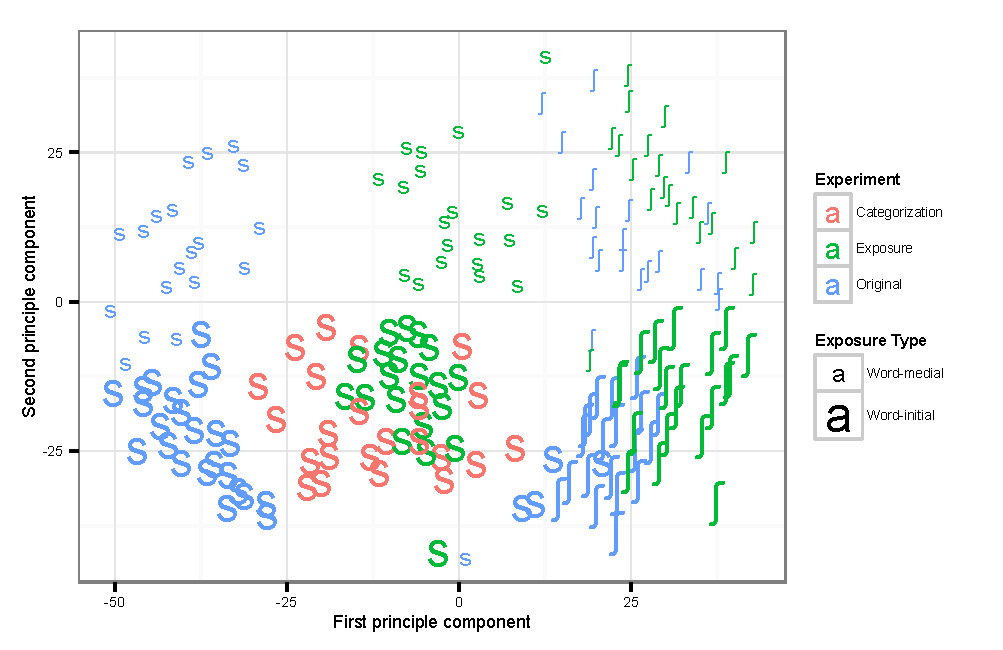
\includegraphics[width=\textwidth]{graphs/exp1_mds}
\end{center}
\end{figure*}

\subsubsection{Experiment design}

Participants were assigned to one of four groups from a 2x2 between-subject factorial design.
The first factor was the position of the ambiguous sibilant in the exposure words (Exposure Type: Word-initial versus Word-medial) and the second factor was whether participants were given additional instructions about the sibilant (Attention: Attention versus No Attention).
Two of the groups of participants were exposed to only critical items that began with /s/ (Word-initial) and the other two were exposed to only critical items that had an /s/ in the onset of the final syllable (Word-medial).
This gave a consistent 200 trials in all exposure phases with identical control and filler items for all participants. 
Participants in half the groups (Attention) received additional instructions that the speaker's ``s'' sounds were sometimes ambiguous, and to listen carefully to ensure correct responses in the lexical decision.
Participants in the control experiment completed only the categorization task.

\subsubsection{Procedure}

Participants in the experimental conditions completed an exposure task and a categorization task in E-Prime \citep{PsychologySoftwareTools2012}.  
Exposure was a lexical decision task, where participants heard auditory stimuli and were instructed to respond with either ``word'' if they thought what they heard was a word or ``nonword'' if they did not think it was a word.  
The buttons corresponding to ``word'' and ``nonword'' were counterbalanced across participants. Trial order was pseudorandom, with no critical or control items appearing in the first six trials and no critical or control trials in a row \citep[following][]{Reinisch2013}.
For each trial, a blank screen was shown for 500 ms, and then the two responses and their corresponding buttons on the button box were shown (i.e. ``word'' and ``1'' on one side of the screen and ``nonword'' and ``5'' on the other side of the screen).
The auditory stimulus was played 500 ms following the presentation of the response options.
Participants had 3000 ms from the onset of the auditory stimulus to respond.
Feedback about whether a response was detected was given once a button was pressed or the 3000 ms had elapsed and was shown for 500 ms before the following trial began.
Every 50 trials participants were given a break and the next trial did not start until the participant pressed a button.

In the categorization task, participants heard an auditory stimulus and had to categorize it as one of two words, differing only in the onset sibilant, i.e. \emph{sin} or \emph{shin}.  
The buttons corresponding to the words were counterbalanced across participants.  
The six most ambiguous steps of the minimal pair continua were used with seven repetitions each, giving a total of 168 trials.
Each trial proceeded similarly to exposure.
A blank screen was displayed for 500 ms, followed by the response screen for 500 ms (i.e. ``sin'' and ``1'' on one side, ``shin'' and ``5'' on the other) before the auditory stimulus was presented.
Participants had 3000 ms from the onset of the auditory stimulus to respond and feedback about whether the response was detected was shown for 1500 ms.
Participants were given a break every 40 trials, except after 160 trials, as that would leave eight trials in the rest of the experiment.

Participants were given oral instructions explaining both tasks at the beginning of the experiment to remove experimenter interaction between exposure and categorization.
Written instructions were presented to participants at the beginning of each task as well.
The instructions for the exposure task given to participants assigned to an Attention condition included explicit reference to the modified sibilants.
Participants were told that ``this speaker's `s' sound is sometimes ambiguous'' and instructed to ``listen carefully so as to choose the correct response.''

\subsubsection{Analysis}

Perceptual learning effects are assessed through logistic mixed-effects models of the categorization task data.
A responses were coded as 1 for /s/ responses and 0 for /\textesh/ responses.
Positive significant estimates therefore indicate higher likelihood of /s/ response across categorization.
Thus, positive significant effects are indicative of perceptual learning, as higher likelihood of /s/ response is associated with an expanded /s/ category.

Deviance contrast coding is used for all two-level independent variables, so the intercept of the model represents the grand mean.
Main effects for factors are calculated with other factors held at their average value, rather than at an arbitrary reference level.
For any factors that have three levels, treatment (dummy) contrasts are used with an appropriate reference level to aid interpretation.
Numeric independent variables were centered prior to inclusion in models.
While the step of the continua is sampled from six discrete levels, it is entered as a numeric variable in the models to reduce the complexity of models.
Graphs of categorization results show continua step as categorical factor to aid interpretation.

For categorization models, Continuum was a random effect.
However, there were only four minimal pair continua used in the categorization, so the random effect status may not be warranted.
The estimates for the continua effects are likely not very reliable, but differences between continua are not the principle question being investigated.
Use of a by-Continuum random effect structure with maximal random slopes allowed for estimation of the fixed effects that are not driven by one particular minimal pair continuum.

\subsection{Results}

\subsubsection{Control experiment}

Responses with reaction times less than 200 ms or greater than 2500 ms were excluded from analyses \citep[following][]{Reinisch2013}. 
A logistic mixed effects model was fit with Subject and Continuum as random effects and Step as a fixed effect with by-Subject and by-Continuum random slopes for Step. 
The intercept was not significant ($\beta = 0.43, SE = 0.29, z = 1.5, p = 0.13$), indicating that control participants did not differ significantly from the pretest participants.
Step was significant ($\beta = -2.61, SE = 0.28, z = -9.1, p < 0.01$), with higher steps (more /\textesh/-like) responded to more as /\textesh/.
Results from the control experiment are shown in Figure~\ref{fig:exp1categ} and all other categorization results as a reference point for interpreting the figures.

\subsubsection{Exposure}

Performance on the exposure task was high overall: 92\% of the filler words were correctly accepted and 89\% of nonwords were correctly rejected.  
Trials with nonword stimuli and responses faster than 200 ms or slower than 2500 ms were excluded from further analysis. 
A logistic mixed-effects model with accuracy as the dependent variable was fit with fixed effects for Trial (0-200), Trial Type (Filler, /s/, and /\textesh/), Attention (No Attention and Attention), Exposure Type (Word-Initial and Word-Medial), and their interactions.   
Trial Type was coded using treatment (dummy) coding, with Filler as the reference level.  
Deviance contrast coding was used for Exposure Type (Word-initial = 0.5, Word-medial = -0.5) and Attention (No attention = 0.5, Attention = -0.5).
The random effect structure was as maximally specified as possible with random intercepts for Subject and Word, and by-Subject random slopes for Trial, Trial Type, and their interactions and by-Word random slopes for Attention, Exposure Type, and their interactions. 

A significant fixed effect was found for Trial Type of /s/ versus Filler ($\beta = -2.13, SE = 0.31, z = -6.8, p < 0.01$), as participants were less likely to endorse words containing the modified /s/ category as compared to filler words.
However, there was a significant interaction between Trial and Trial Type of /s/ versus Filler ($\beta = -0.45, SE = 0.14, z = 3.1, p = 0.01$), so the differences in accuracy between words with /s/ and filler words diminished over time.
There was also a significant main effect of Attention ($\beta = -0.57, SE = 0.28, z = -2.0, p = 0.04$), indicating that participants were more accurate at identifying words in the Attention condition compared to the No Attention condition.
However, there was a marginal interaction between Attention and Trial Type of /s/ versus Filler ($\beta = 0.72, SE = 0.39, z = 1.8, p = 0.06$), suggesting that attention only increased accuracy for words not containing the modified /s/ category.
Figure~\ref{fig:exp1exposeacc} shows within-subject mean accuracy across exposure, with Trial in four blocks.

\begin{figure*}[!ht]
\caption{Within-subject mean accuracy for words in the exposure phase of Experiment 1, separated out by Trial Type (Filler, /s/, and /\textesh/). Error bars represent 95\% confidence intervals.}
\label{fig:exp1exposeacc}
\begin{center}
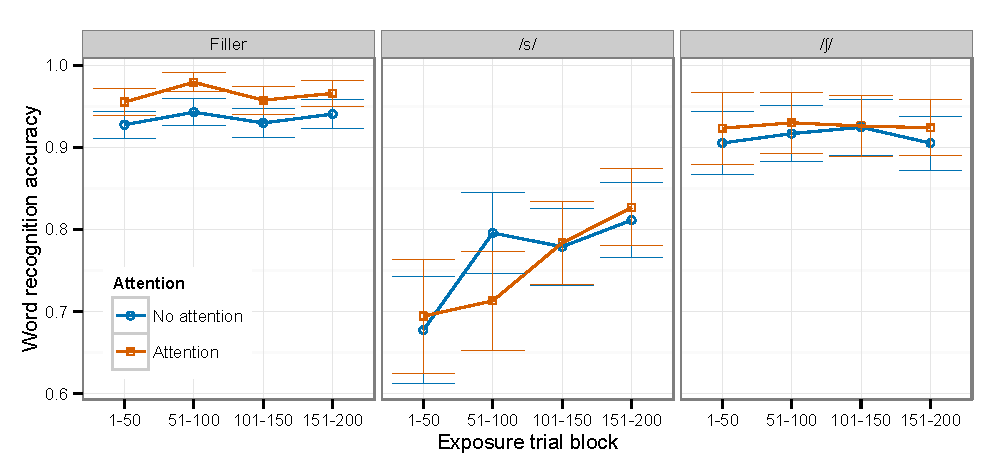
\includegraphics[width=\textwidth]{graphs/exp1_expacc}
\end{center}
\end{figure*}

A linear mixed-effects with logarithmically-transformed reaction time as the dependent variable was fit with identical fixed effect and random effect structure as the logistic model for accuracy.
Significant effects were found for Trial Type of /s/ versus Filler ($\beta = 0.71, SE = 0.07, t = 10.8$) and the interaction between Trial and Trial Type of /s/ versus Filler ($\beta = -0.08, SE = 0.02, t = -3.1$).  
These effects follow the pattern found in the accuracy model, where participants begin with slower reaction times to words with /s/, but over time this difference between words /s/ and filler words lessens.  
Figure~\ref{fig:exp1exposert} shows within-subject mean reaction time across exposure, with Trial in four blocks.

\begin{figure*}[!ht]
\caption{Within-subject mean reaction time to words in the exposure phase of Experiment 1, separated out by Trial Type (Filler, /s/, and /\textesh/). Error bars represent 95\% confidence intervals.}
\label{fig:exp1exposert}
\begin{center}
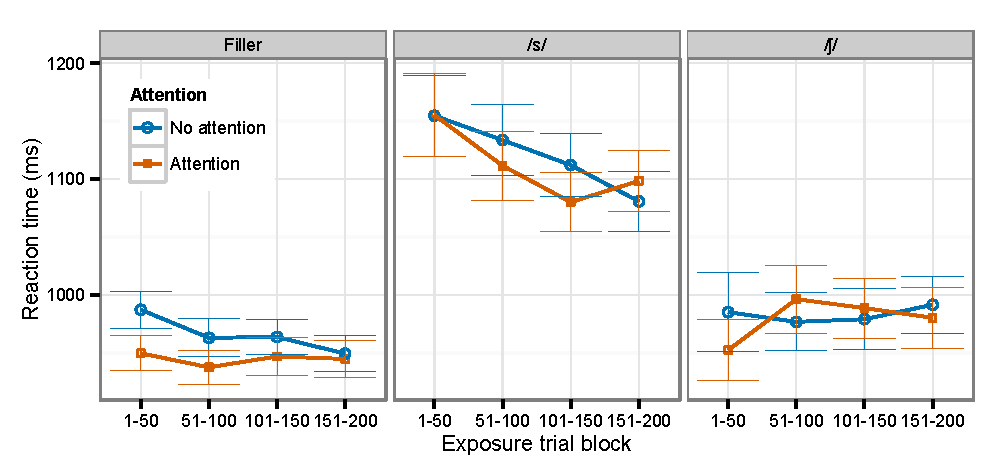
\includegraphics[width=\textwidth]{graphs/exp1_exprt}
\end{center}
\end{figure*}

\subsubsection{Categorization}

Responses with reaction times less than 200 ms or greater than 2500 ms were excluded from analyses. 
Two participants were excluded because their initial estimated cross-over point for the continuum lay outside of the 6 steps presented.  
A logistic mixed effects model was constructed with Subject and Continuum as random effects and a by-Subject random slope for Step and by-Continuum random slopes for Step, Attention, Exposure Type, and their interactions. 
Fixed effects for the model were Step, Exposure Type, Attention, and their interactions.  
Deviance contrast coding was used for Exposure Type (Word-initial = 0.5, Word-medial = -0.5) and Attention (No attention = 0.5, Attention = -0.5).
An /s/ response was coded as 1 and an /\textesh/ response as 0.

\begin{figure*}[!ht]
\caption{Proportion /s/ response along the 6 step continua as a function of Exposure Type and Attention in Experiment 1.    Error bars represent 95\% confidence intervals.}
\label{fig:exp1categ}
\begin{center}
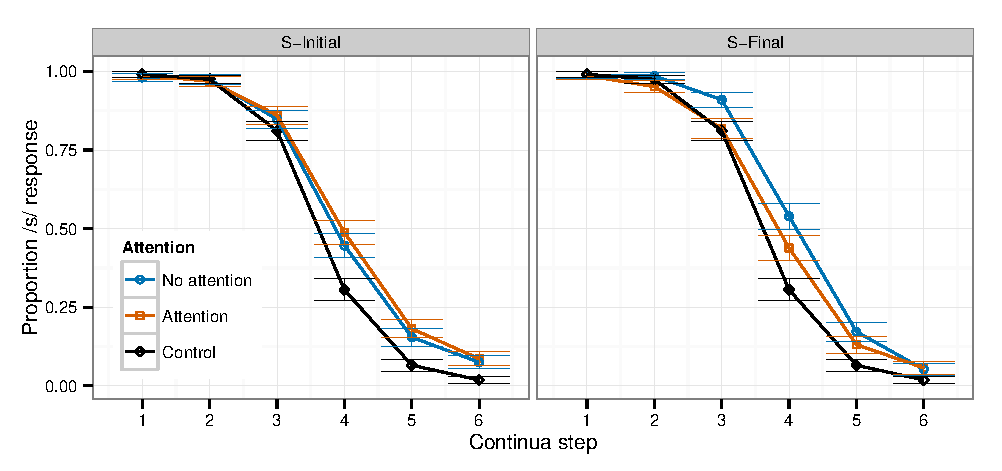
\includegraphics[width=\textwidth]{graphs/exp1_categresults}
\end{center}
\end{figure*}

There was a significant effect for the intercept ($\beta = 0.76, SE = 0.22, z = 3.3, p < 0.01$), indicating that participants categorized more of the continua as /s/ in general.  
This is evidence of learning compared to participants in the control experiment.
There was also a significant main effect of Step ($\beta = -2.14, SE = 0.15, z = -14.2, p < 0.01$), and a significant interaction between Exposure Type and Attention ($\beta = -0.93, SE = 0.45, z = -2.04, p = 0.04$).  The results are visualized Figure~\ref{fig:exp1categ}.
When exposed to a modified /s/ category at the beginning of words, participants show a general expansion of the /s/ category with no difference in behavior induced by the attention manipulation.  
However, when the exposure is to ambiguous /s/ tokens later in the words, we can see differences in behavior beyond the general /s/ category expansion.  
Participants not warned of the speaker's ambiguous tokens categorized more of the continua as /s/ compared to those who were warned of the speaker's ambiguous /s/ productions.

\subsection{Discussion}

The condition that showed the largest perceptual learning effect was the one most biased toward a comprehension-oriented attentional set.
Participants exposed to the modified /s/ category in the middle of words and with no explicit instructions about /s/ had larger perceptual learning effects than any of the other conditions.
The other conditions showed roughly equivalent sizes of perceptual learning, suggesting that there was not a compounding effect of explicit attention and word position.
That is, the comprehension-oriented nature of the primary task still exerts an effect on attentional set selection, and a significant perceptual learning effect was found on novel words.

The findings of this experiment do not support the predictions of a purely gain-based mechanism for attention, such as the one posited by \citet{Clark2013}.
If attention functioned as a gain mechanism, increasing the weight of error signals generated by mismatches between expectations and incoming signals, we should expect to see greater perceptual learning when listeners were instructed to attend to the speaker's /s/ sounds.
Instead, the opposite was found.
Participants told to attend to the speaker's /s/ sounds showed smaller perceptual learning effects.
The nature and valency of the instructions may affect the outcome of attention.
In this experiment, the instructions regarding /s/ were phrased to suggest that the ambiguity of the speaker's ``s'' could harm accuracy.
If the valency of the attention were more positive, such as giving an explanation for the cause of ambiguity, then explicit instructions might cause a different pattern of effect.
For a gain-based mechanism, however, valency of attention is not predicted to affect attention, but rather attention always increasing the gain of error signals.
If valency of the instructions does change behavior, then it would be another mark against a gain mechanism.

In addition to the perceptual learning effects of the categorization phase, the exposure phase also demonstrates learning.  
In the initial trials, words with a modified /s/ are responded to more slowly and less accurately, but over the course of exposure, both reaction times and accuracy approach those of filler and unmodified /\textesh/ words.
Interestingly, only the attention manipulation had an effect on exposure performance, with participants attending to the /s/ category responding more accurately overall.
Exposure Type did not significantly influence accuracy or reaction time in the exposure task.

Much of the literature on perceptual learning in speech perception focuses on the issue of generalization and specificity.
For instance, listeners have been shown to generalize across speakers more if the exposure speaker's modified category happens to be within the range of variation of the categorization speaker's stimuli \citep{Eisner2005,Kraljic2005}.
Additionally, many perceptual learning studies artificially enhance the similarity between exposure tokens and categorization tokens, for instance splicing the maximally ambiguous step of the categorization continuum into exposure words \citep{Norris2003}.
Because exposure-specificity plays such a large role in perceptual learning, it is natural to consider whether the greater perceptual learning effects in some conditions arise due to greater similarity to the exposure stimuli.
However, as shown in Figure~\ref{fig:exp1mds}, Word-medial exposure tokens are acoustically farther from the categorization tokens than the Word-initial exposure tokens.  
Even if auditory similarity of /s/ across exposure and categorization played any role, it was still overridden by the experimental manipulations.

In this experiment I used a similar method for exposure stimuli selection as \citet{Reinisch2013}, but used a threshold of 50\% word response rate in the pretest as the cutoff rather than 70\%.
With their 70\% stimuli, Reinisch and colleagues report word endorsement rates that consistently exceeded 85\%.
In contrast, Experiment 1 used 50\% as the threshold and had correspondingly lower word endorsement rates (mean = 76\%, SD = 22\%).  
Despite the lower word endorsement rates and the less canonical stimuli used, perceptual learning effects remained robust.
This raises the question, can perceptual learning occur from a modified category even more atypical than the one used in this experiment?
More atypical categories should be more salient and induce more a perception-oriented attentional set, and therefore result in smaller perceptual learning effects.
In Experiment 2, we test whether a comprehension-oriented attentional set can be maintained despite the category atypicality triggering perception-oriented attentional sets.

\section{Experiment 2}

Experiment 2 uses stimuli that are farther from the canonical productions of the critical exposure tokens containing /s/.

\subsection{Methodology}

\subsubsection{Participants}

A total of 127 participants from the UBC population completed the experiment and were compensated with either \$10 CAD or course credit.  
The data from 31 non-native speakers of English were excluded from the analyses.
This left data from 96 participants for analysis.

\subsubsection{Materials}

Experiment 2 used the same items as Experiment 1, except that the step along the /s/-/\textesh/ continua chosen as the ambiguous sound had a different threshold.  
For this experiment, 30\% identification as the /s/ word was used the threshold. The average step chosen for /s/-initial words was 7.3 ($SD = 0.8$), and for /s/-medial words the average step was 8.9 ($SD = 0.9$).  
The list of steps chosen for Word-initial and Word-medial target stimuli are in Tables~\ref{tbl:exp2srespinitial} and~\ref{tbl:exp2srespfinal}, respectively.  
Note that for several stimuli, the same steps are used for both Experiment 1 and 2.
There were large jumps in proportion /s/ response between steps for the continua for those stimuli.
However, the key aspect of the stimuli is the distribution of the /s/ category as a whole, and not the individual steps.

\begin{table}[ht]
\caption{Step chosen for each Word-initial stimulus in Experiment 2 and the proportion /s/ response in the pretest}
\label{tbl:exp2srespinitial}
\centering
\begin{tabular}{ccc}
\toprule
 Word & Step chosen & Proportion /s/ response \\
\midrule
 ceiling & 8 & 0.20 \\
 celery & 7 & 0.30 \\
 cement & 7 & 0.26 \\
 ceremony & 8 & 0.39 \\
 saddle & 8 & 0.25 \\
 safari & 7 & 0.21 \\
 sailboat & 7 & 0.35 \\
satellite & 8 & 0.30 \\
 sector & 6 & 0.39 \\
 seminar & 7 & 0.33 \\
 settlement & 8 & 0.35 \\
 sidewalk & 7 & 0.30 \\
 silver & 7 & 0.21 \\
 socket & 7 & 0.30 \\
 sofa & 7 & 0.26 \\
 submarine & 9 & 0.32 \\
 sunroof & 6 & 0.39 \\
 surfboard & 8 & 0.25 \\
 syrup & 6 & 0.37 \\
\midrule
Average  & 7.3 & 0.30 \\

\bottomrule
\end{tabular}
\end{table}


\begin{table}[ht]
\caption{Step chosen for each Word-medial stimulus in Experiment 2 and the proportion /s/ response in the pretest}
\label{tbl:exp2srespfinal}
\centering
\begin{tabular}{ccc}
\toprule
 Word & Step chosen & Proportion /s/ response \\
\midrule
 carousel & 8 & 0.25 \\
 castle & 9 & 0.25 \\
 concert & 10 & 0.30 \\
 croissant & 8 & 0.20 \\
 currency & 9 & 0.30 \\
 cursor & 11 & 0.30 \\
 curtsy & 9 & 0.26 \\
 dancer & 8 & 0.26 \\
 dinosaur & 9 & 0.39 \\
 faucet & 8 & 0.25 \\
 fossil & 8 & 0.30 \\
 galaxy & 10 & 0.26 \\
 medicine & 9 & 0.30 \\
missile & 10 & 0.30 \\
monsoon & 9 & 0.15 \\
 pencil & 8 & 0.37 \\
 pharmacy & 9 & 0.39 \\
 tassel & 8 & 0.35 \\
 taxi & 10 & 0.35 \\
 whistle & 9 & 0.35 \\
\midrule
 Average  & 8.9 & 0.29 \\

\bottomrule
\end{tabular}
\end{table}

Multidimensional scaling was employed to assess the distributions of the stimuli used in Experiment 2.
A similar pattern is found for Experiment 2 as Experiment 1.
The axes remain the same as before, with the first dimension corresponding to differences between sibilants, and the second dimension corresponding to differences in word position.
The original productions, categorization tokens, and /\textesh/ tokens in Figure~\ref{fig:exp2mds} are identical to those shown in Figure~\ref{fig:exp1mds}, but the exposure token distribution is shifted towards the /\textesh/ distribution.  
In the Word-medial position, the distributions of /s/ and /\textesh/ are close to overlapping, and in the Word-initial position, they are still separated, but closer than in the stimuli for Experiment 1.


\begin{figure*}[ht]
\caption{Multidimensional scaling of the acoustic distances between the sibilants of original productions, categorization tokens and the exposure tokens in Experiment 2.  Categorization and exposure tokens were synthesized from the original productions using STRAIGHT \citep{Kawahara2008}.}
\label{fig:exp2mds}
\begin{center}
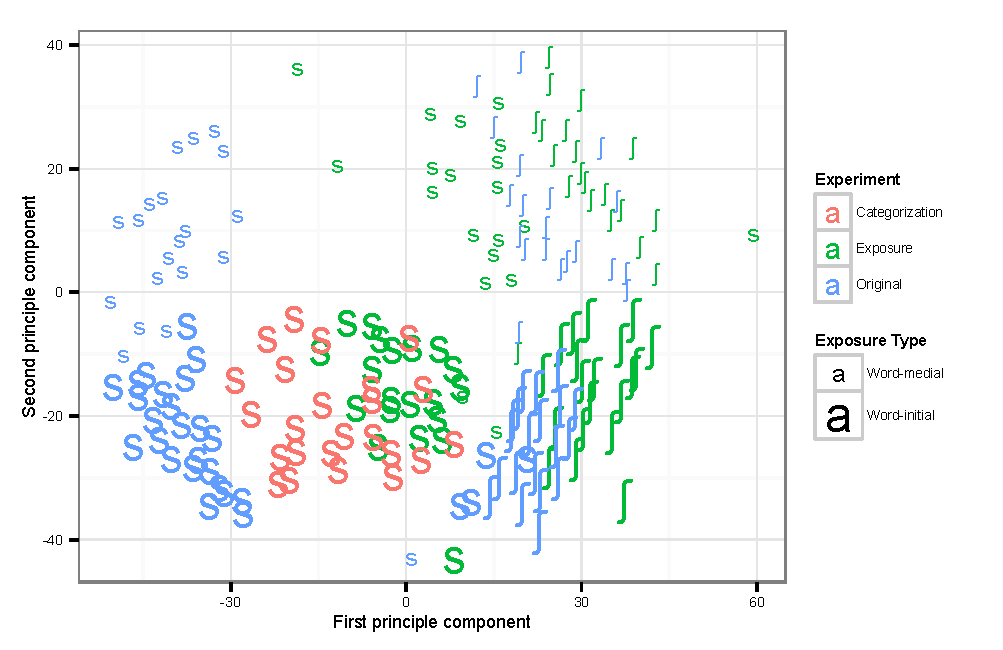
\includegraphics[width=\textwidth]{graphs/exp2_mds}
\end{center}
\end{figure*}

\subsubsection{Procedure}

The procedure and instructions were identical to those of Experiment 1.

\subsubsection{Analysis}

Response data and factors were transformed and analyzed in the same way as in Experiment 1.

\subsection{Results}

\subsubsection{Exposure}

Trials with nonword stimuli and responses faster than 200 ms or slower than 2500 ms were excluded from analysis. 
Performance on the exposure task was as high, with accuracy on filler trials averaging 92\%.  
A logistic mixed-effects model with accuracy as the dependent variable and a linear mixed-effects model with reaction time (logarithmically-transformed) as the dependent variable were fit with identical specifications as Experiment 1.

In the logistic mixed-effects model of accuracy, a significant fixed effect was found for Trial Type of /s/ versus Filler ($\beta = -3.56, SE = 0.31, z = -11.4, p < 0.01$), with participants less likely to respond that an item was a word if it contained the modified /s/ category.
There was a significant interaction between Trial and Trial Type of /s/ versus Filler ($\beta = -0.29, SE = 0.11, z = 2.5, p < 0.01$) and between Trial and Trial Type of /\textesh/ versus Filler ($\beta = -0.33, SE = 0.16, z = -2.0, p = 0.04$).  
These interactions indicate that participants became more likely to endorse words with modified /s/ productions over time, but also became less accurate on words containing /\textesh/.  
Figure~\ref{fig:exp2exposeacc} shows within-subject mean accuracy across exposure, with Trial in four blocks.

%Trial Type of /s/ versus Filler and Exposure Type ($\beta = 0.97, SE = 0.53, z = 1.8, p = 0.07$) 

\begin{figure*}[!ht]
\caption{Within-subject mean accuracy in the exposure phase of Experiment 2, separated out by Trial Type (Filler, /s/, and /\textesh/). Error bars represent 95\% confidence intervals.}
\label{fig:exp2exposeacc}
\begin{center}
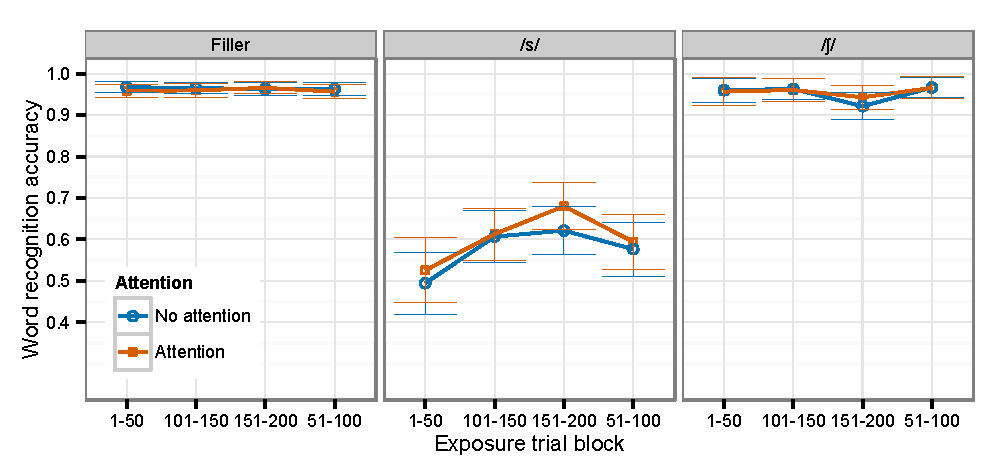
\includegraphics[width=\textwidth]{graphs/exp2_expacc}
\end{center}
\end{figure*}

In the linear mixed-effects model of reaction time, significant effects were found for Trial Type of /s/ versus Filler ($\beta = 0.94, SE = 0.07, t = 14.4$), indicating that reaction times were slower for words containing the modified /s/ category.
Also significant was the interaction between Trial and Trial Type of /\textesh/ versus Filler ($\beta = 0.07, SE = 0.02, t = 3.4$).
However, there was no the interaction between Trial and Trial Type of /s/ versus Filler ($\beta = -0.02, SE = 0.02, t = -0.8$). 
This indicates that reaction time remained relatively stable for words containing the modified /s/ category, but lengthened for words containing the /\textesh/ control.  
There was a marginal effect for Trial Type of /\textesh/ versus Filler ($\beta = 0.14, SE = 0.07, t = 1.9$), indicating that words with /\textesh/ tended to be responded to more slowly than filler times.
Finally, there was a marginal effect of Exposure Type ($\beta = 0.17, SE = 0.09, t = 1.9$), indicating that words in the Word-medial condition tended to be responded to faster.
Figure~\ref{fig:exp2exposert} shows within-subject mean reaction time across exposure, with Trial in four blocks.

%itemtypeSH ($\beta = 0.14, SE = 0.07, t = 1.9$)
%exposure type ($\beta = 0.17, SE = 0.09, t = 1.9$)

\begin{figure*}[!ht]
\caption{Within-subject mean reaction time in the exposure phase of Experiment 2, separated out by Trial Type (Filler, /s/, and /\textesh/). Error bars represent 95\% confidence intervals.}
\label{fig:exp2exposert}
\begin{center}
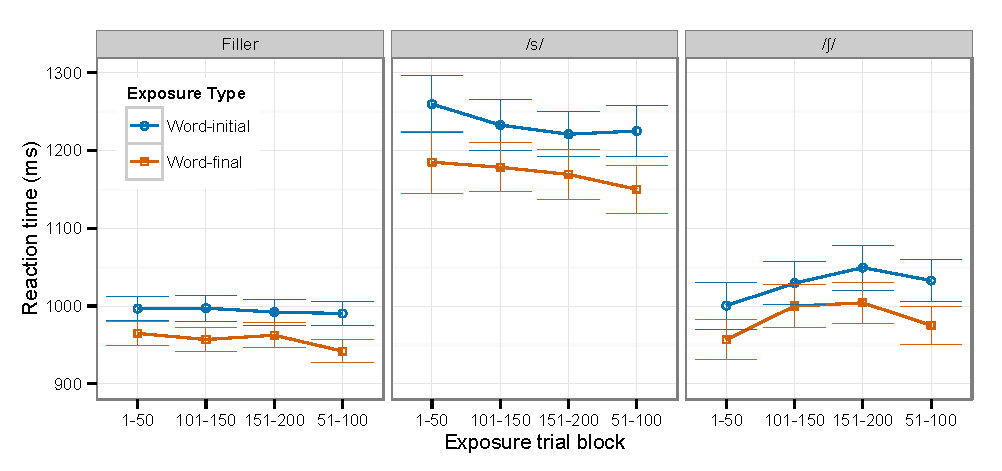
\includegraphics[width=\textwidth]{graphs/exp2_exprt}
\end{center}
\end{figure*}

\subsubsection{Categorization}

Responses with reaction times less than 200 ms or greater than 2500 ms were excluded from analyses. 
Two participants were excluded because their initial estimated cross-over point for the continuum lay outside of the 6 steps presented.  
A logistic mixed effects model was constructed with identical specification as Experiment 1.

\begin{figure*}[!ht]
\caption{Proportion /s/ response along the 6 step continua as a function of Exposure Type and Attention in Experiment 2. Error bars represent 95\% confidence intervals.}
\label{fig:exp2categ}
\begin{center}
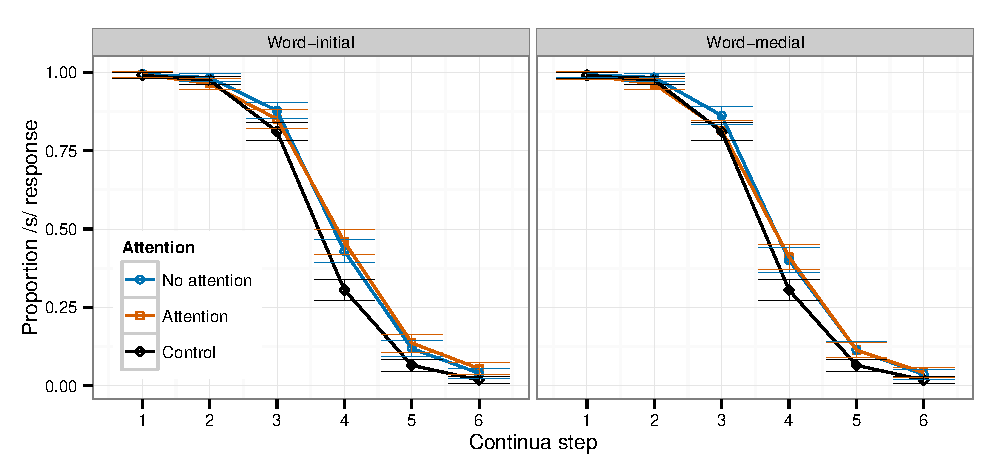
\includegraphics[width=\textwidth]{graphs/exp2_categresults}
\end{center}
\end{figure*}

There was a significant effect for the Intercept ($\beta = 0.60, SE = 0.26, z = 2.3, p = 0.02$), indicating that participants categorized more of the continua as /s/ in general. 
 There was also a significant main effect of Step ($\beta = -2.51, SE = 0.19, z = -13.1, p < 0.01$).  
Unlike in Experiment 1, there were no other significant effects, suggesting that participants across conditions had similar perceptual learning effects.
These results are shown in Figure~\ref{fig:exp2categ}

\section{Grouped results across experiments}

To see what degree the stimuli used had an effect on perceptual learning, the data from Experiment 1 and Experiment 2 were pooled and analyzed identically as above, but with Experiment and its interactions as additional fixed effects.  
In the logistic mixed effects model, there was significant main effects for Intercept ($\beta = 1.00, SE = 0.36, z = 2.7, p < 0.01$) and Step ($\beta = -2.64, SE = 0.21, z = -12.1, p < 0.01$), a significant two-way interaction between Experiment and Step ($\beta = 0.51, SE = 0.20, z = 2.5, p = 0.01$), and a marginal four-way interaction between Step, Exposure Type, Attention and Experiment ($\beta = 0.73, SE = 0.42, z = 1.7, p = 0.08$).  
These results can be seen in Figure~\ref{fig:exp12categ}.  
The four-way interaction can be seen in Word-medial/No Attention conditions across the two experiments, where Experiment 1 has a difference between the Attention and No Attention condition, but Experiment 2 does not.  
The two-way interaction between Experiment and Step and the lack of a main effect for Experiment suggests that while the category boundary was not significantly different across experiments, the slope of the categorization function was.

\begin{figure*}[!ht]
\caption{Proportion /s/ response along the 6 step continua as a function of Exposure Type and Attention in Experiment 1 and Experiment 2. Error bars represent 95\% confidence intervals.}
\label{fig:exp12categ}
\begin{center}
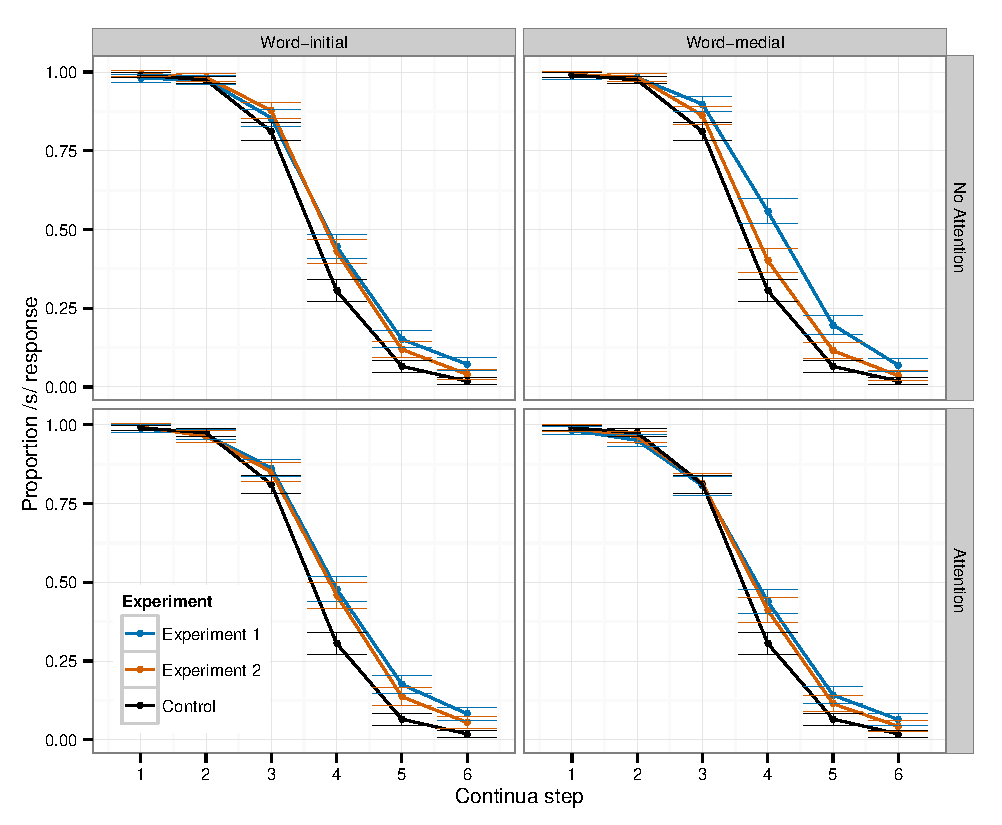
\includegraphics[width=\textwidth]{graphs/exp12_categresults}
\end{center}
\end{figure*}

In previous research, a link has been shown between the proportion of word endorsement for exposure tokens and the size of perceptual learning effects \citep{Scharenborg2013}.
Listeners who endorsed more of exposure tokens as words showed a larger perceptual learning effect.
To assess such a link in the current experiments a logistic mixed-effects model was constructed identically as above, but with participants' word endorsement rate of target /s/ words as an additional fixed effect, along with its interactions with all other fixed effects.
Word endorsement rate was calculated as the ratio of the number of word responses by the total number of /s/ trials.
For analysis, the word endorsement rates were analyzed using an arcsine transformation.
Word endorsement rate was significant ($\beta = 1.55, SE = 0.38, z = 4.1, p < 0.01$), finding the same effect as previous work.
Participants who endorsement more exposure tokens showed larger perceptual learning effects.
Word endorsement rate significantly interacted with Step ($\beta = 0.63, SE = 0.24, z = 2.6, p < 0.01$) and was involved in a marginal  interaction with Step, Attention and Experiment ($\beta = -1.79, SE = 0.94, z = -1.8, p = 0.06$).

To better investigate the nature of the four-way interaction, word endorsements were correlated with estimated cross-over points by participant.  
Cross-over points are where a participant's perception switches from predominantly /s/ to predominantly /\textesh/.
The cross-over point was determined from the Subject random intercept and the by-Subject random slope of Step in a simple model containing only those random effects, similar by-Continuum random effects, and a fixed effect for Step \citep{Kleber2012}. 
Scatter plots of word endorsement rate and cross-over point across all experimental conditions are shown in Figure~\ref{fig:exp12xover}.
In general there is a positive correlation between word endorsement rate in the exposure phase and the cross-over point from /s/ to /\textesh/ in the categorization phase.
Participants in the Experiment 1 who were exposed to more typical /s/ stimuli showed a stronger correlation across conditions than participants in Experiment 2 who were exposed to a more atypical /s/ category.
An ANOVA with a dependent variable of word response rate with Exposure Type, Attention, Experiment, and their interactions revealed only a significant difference in endorsement rates for Experiment ($F(1, 187) = 26.8, p < 0.01$).  
Experiment 1 had a mean word endorsement rate of 75\% (SD = 23\%) and Experiment 2 had a mean endorsement rate of 58\% (SD = 27\%).

\begin{figure*}[!ht]
\caption{Correlation of cross-over point in categorization with the proportion of word responses to critical items containing an ambiguous /s/ token in Experiments 1 and 2.}\label{fig:exp12xover}
\begin{center}
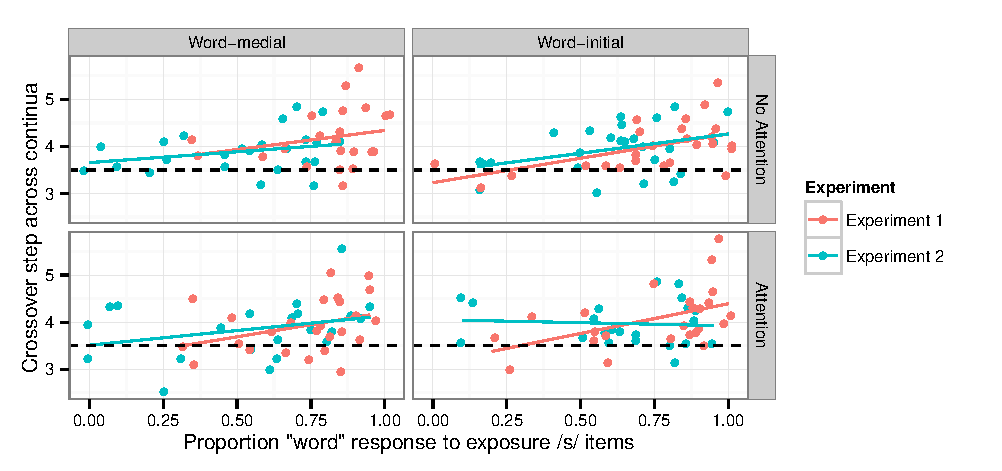
\includegraphics[width=\textwidth]{graphs/exp12_xoverwordresp}
\end{center}
\end{figure*} 

In Experiment 1, the strongest correlations between word endorsement rate and cross-over point are seen in the Word-initial conditions (Attention: $r = 0.46, t(22) = 2.4, p = 0.02$; No Attention: $r = 0.45, t(22) = 2.4, p = 0.02$), with the next strongest, and more marginal, correlation in Word-medial/Attention condition ($r = 0.39, t(23) = 2.0, p = 0.06$).  The condition for which the most perceptual learning was observed (Word-medial/No Attention) actually has the weakest relationship ($r = 0.32, t(21) = 1.5, p = 0.13$).

In Experiment 2, the strongest correlation is in the Word-initial/No Attention condition ($r = 0.40, t(23) = 2.1, p = 0.05$), with two trending correlations for the Word-medial conditions (Attention: $r = 0.33, t(20) = 1.6, p = 0.12$; No Attention: $r = 0.27, t(22) = 1.3, p = 0.20$).  Finally, the correlation for the Word-initial/Attention condition is not significant ($r = -0.05, t(20) = -0.2, p = 0.82$).

\section{General discussion}


The perceptual learning effects found in Experiment 1 and 2 align with either comprehension-oriented or perception-oriented attentional sets.  
The perception-oriented attentional sets are predicted to exhibit less generalization, similar to what is seen in the psychophysics literature and  in visually-guided perceptual learning in speech perception \citep{Reinisch2014}.
In support of this, participants in Experiment 1 conditions that guided the use of a perception-oriented attentional set (i.e., Attention conditions and Word-initial conditions), showed uniform and modest amounts of perceptual learning.
Those in Experiment 2 who were triggered to use a perception-oriented set based on the category atypicality of the stimuli showed similar modest levels of perceptual learning.
Participants that were not exposed to any triggers towards perception-oriented attentional sets (Experiment 1/ No Attention/ Word-medial) were predicted to use a more comprehension-oriented attentional set which aligns with the task performed.
These participants showed a substantially larger perceptual effect than those bias towards perception-oriented attentional sets.

Compared to Experiment 1, Experiment 2 had a weaker correlation between critical word endorsement rates and cross-over boundary points.
This suggests that although the stimuli used in Experiment 2 were farther from the canonical production, they did not shift the category boundary as much as the stimuli in Experiment 1.  
While neither attention nor position of the ambiguous sound had an effect on the correlation, the distance from the canonical production did.  
This potentially suggests that the degree to which a category is shifted is inverse of the token's distance to the mean.

In Experiment 1, the decreased correlation between word response rate and cross-over point in the condition that saw the largest perceptual learning effects falls out from the proposed attention mechanism.
Comprehension-oriented attentional sets are proposed to update higher, more abstract linguistic representations.
Initial endorsements might shift the boundary more than later endorsements under such an attentional set, which would result in a non-linear relationship between endorsement rate and cross-over point.
Lexically-guided perceptual learning is typically induced with relatively few tokens, usually 20 of 200 total tokens \citep{Norris2003, Reinisch2013}, but as few as 10 modified tokens have been shown to cause perceptual learning \citep{Kraljic2008}.
Under perception-oriented attentional sets, the relationship between endorsement rate and cross-over point may be more linear, with equal updating per endorsement, but each individual instance contributes less than initial comprehension-oriented endorsements.
Visually-guided perceptual learning generally uses hundreds of target tokens with no fillers \citep{Vroomen2007, Reinisch2014}.

The correlation between word response rate in the exposure phase and the category boundary in categorization phase across both experiments has two possible explanations. 
In a causal interpretation between exposure and categorization, as each ambiguous sound is processed and errors propagate, the distribution for that category (for that particular speaker) is updated.
Participants who processed more of the ambiguous sound as an /s/ updated their perceptual category for /s/ more. 
This explanation fits within a Bayesian model of the brain \citep{Clark2013} or a neo-generative model of spoken language processing \citep{Pierrehumbert2002}.  
A non-causal story is also plausible:  the correlation may reveal individual differences on the part of the participants, where some participants are more adaptable or tolerant of variability than others.
These more tolerant listeners then show greater degrees of perceptual adaptation. 
Individual differences in attention-switching control have previously been found to affect perceptual learning \citep{Scharenborg2014}, which supports a non-causal interpretation as well.

As mentioned in the discussion for Experiment 1, the findings do not support a simple gain mechanism for attention \citep[contra][]{Clark2013}.  
In \citet{Yeshurun1998}, attention to areas with finer spatial resolution caused observers to miss larger patterns.  
If attention simply boosted the error signal, attention of all kinds should always be beneficial to perceptual learning.
The findings of these two experiments supports a larger role for attention in a predictive coding framework, which been previously noted in \citet{Block2013}.
The propagation-limiting attention mechanism proposed in this dissertation explains both the findings in the visual domain and the current findings.
Attention to a level of representation causes errors between expectations and observed signals to be resolved and updated at that level.
If attention is more oriented towards comprehension, errors can be propagated to a higher, more abstract level of linguistic representation before updating expectations.

A lexical decision task by default biases a participant towards a comprehension-oriented attentional set.
The experimental manipulations promoted perception-oriented attentional sets that attenuated generalized perceptual learning effects.
To fully examine the use of perception- and comprehension-oriented attentional sets in perceptual learning, manipulations that induce comprehension-oriented attentional sets are necessary.
In the following chapter, such a manipulation is implemented through increasing linguistic expectations with semantic predictability.




